\subsubsection {}
\label{sec:analysis:research:backArch:microservices}

Микросервисная архитектура предлагает рассматривать программное средство как набор слабо связанных сервисов, взаимодействующих друг с другом. Каждый сервис реализует фокусированный набор связанных функций. Например, программное средство может содержать сервисы для авторизации, отправки сообщений, пуш-уведомлений.

Сервисы могут общаться при помощи как синхронных, так и асинхронных протоколов, часто выбор ложится на \gls{http}/REST. Такой подход позволяет разрабатывать и разворачивать сервисы независимо друг от друга, каждый сервис имеет собственную базу данных, консистентность данных между сервисами поддерживается при помощи паттерна Saga\cite{microservices:ms}.

На рисунке \ref{sec:analysis:research:arch:back:micro} представлен пример организации микросервисного ПС.

\begin{figure}[h]
  \centering
    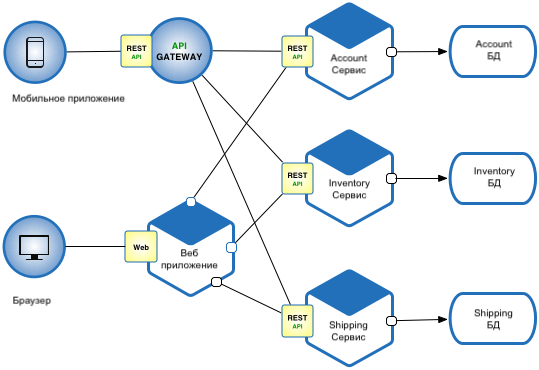
\includegraphics[width=1\textwidth]{inc/img/backend-micro.png}
  \caption{Пример организации монолитного серверного ПС}
  \label{sec:analysis:research:arch:back:micro}
\end{figure}

Очевидными плюсами микросервисного подхода являются:

\begin{enumerate}
	\item \emph{Тестируемость} -- небольшие сервисы проще тестировать в изолированной среде.
	\item \emph{Скорость развёртывания} -- небольшой сервис разворачивается намного быстрее полноценного ПС.
	\item \emph{Модульность} -- микросервисная архитектура значительно упрощает разделение сотрудников на команды.
	\item \emph{Меньший порог входа} -- разработчику нужно разбираться только с одним небольшим сервисом.
	\item \emph{Скорость разработки} -- отсутствие неявных зависимостей, скорость развёртывания и скорость работы \gls{ide} положительно сказываются на продуктивности разработчиков.
	\item \emph{Повышенная отказоустойчивость} -- выход из строя одного сервиса не выведет из строя всё ПС.
	\item \emph{Гибкость масштабирования} -- разработчики получают возможность масштабировать отдельно сервисы.
	\item \emph{Гибкость в выборе технологического стека} -- каждый сервис может быть разработан, используя собственный технологический стек, переход на новую технологию можно выполнять поэтапно.
\end{enumerate}

Однако, микросервисная архитектура значительно повышает общую сложность системы, вводя дополнительную работу для программистов:

\begin{enumerate}
	\item \emph{Отсутствие поддержки со стороны \gls{ide}} -- если перед разработчиком стоит задача, которая предполагает изменение нескольких сервисов -- \gls{ide} будет неспособна работать над несколькими проектами одновременно.
	\item Появляется необходимость разработки и поддержки протокола общения между сервисами.
	\item Перед разработчиками появляются задачи координации сервисов, аггрегации запросов.
	\item \emph{Усложнённый процесс запуска всего ПС} -- для запуска всего ПС требуется развернуть каждый сервис отдельно.
	\item \emph{Повышенное потребление ресурсов} -- каждый сервис является отдельным процессом, поэтому ресурсы, которые тратятся на поддержку работоспособности процесса увеличиваются на количество сервисов.
\end{enumerate}

% Так как каждый сервис имеет собственную базу данных, а часто бизнес-логика требует работы сразу нескольких сервисов, стоит рассмотреть механизмы для аггрегации запросов между сервисами и поддержки консистентности состояния.

% -- Api Composition
% -- Saga pattern